
%%
%% This file creates the Item, ItemPacket, ItemFold, ItemEnvelope, and
%% ItemLabel datatypes, and creates macros for each.  These are for
%% various types of in-game items.
%%
%%%%%


%%%%%
%% Item macros are for normal item cards.
\DECLARESUBTYPE{Item}{TransElement}
\PRESETS{Item}{
  \FD\MYtext	{} %% longer text of item
  \FD\MYmark	{} %% possible contents of shaded ``mark'' on card
  \FD\MYbulky	{0} %% potential bulkiness
  \FD\MYvalue	{Not Sellable}
  \FD\MYcapacity{N/A} %% potential capacity
  \sd\MYlistmap	{\item\MYname\ifx\MYnumber\empty\else\ (\MYnumber)\fi}
  }


%%%%%
%% \prop
%% \unstash
%% \bulky{<number>}
%% \contain{<number>}
%%
%% \prop inside an Item macro labels the card as a prop.  \unstash
%% labels the card as unstashable.  \bulky{n} labels the card as
%% n-hands bulky.  \contain{n} labels the card with n-hands capacity.
%\def\prop{%
 % \append\MYmark{ ~PROP~ }}
  \def\tinker{%
  \append\MYmark{ ~TINKERABLE~ }}
\def\unstash{%
  \append\MYmark{ ~UNSTASHABLE~ }}
\def\bulky#1{%
  \s\MYbulky{#1}%
  \append\MYmark{\mbox{ ~\MYbulky-Hand~Bulky~ }}}
\def\contain#1{%
  \s\MYcapacity{#1}%
  \append\MYmark{\mbox{ ~\MYcapacity-Hand~Capacity~ }}}
\def\value#1{%
  \s\MYvalue{#1}%
  \append\MYmark{\mbox{ ~Cash value: \MYvalue~ }}}

%%%%%
%% ItemPacket macros are for item cards with an attached packet.
%% They are a subtype of Item.
\DECLARESUBTYPE{ItemPacket}{Item}
\PRESETS{ItemPacket}{
  \F\MYcontents
  }


%%%%%
%% ItemFold macros are for items represented by just a folded packet.
%% They are a subtype of ItemPacket, with the longer text and ``mark''
%% left blank, since they have no actual item card.
\DECLARESUBTYPE{ItemFold}{ItemPacket}
\PRESETS{ItemFold}{
  \s\MYmark{}
  }


%%%%%
%% ItemEnvelope macros are for items represented by just an envelope.
%% They are a subtype of ItemPacket, with the longer text and ``mark''
%% left blank, since they have no actual item card.
\DECLARESUBTYPE{ItemEnvelope}{ItemPacket}
\PRESETS{ItemEnvelope}{
  \s\MYmark{}
  }


%%%%%
%% ItemLabel macros are for small labels that would get used on
%% physreps, e.g. gun labels.  The ``mark'' is left blank, since
%% it isn't used for these.
\DECLARESUBTYPE{ItemLabel}{Item}
\PRESETS{ItemLabel}{
  \s\MYmark{}
  }


%%%%%
%% \icard[<extras>]{<name>}{<number>}{<text>}
%% \specialicard[<extras>]{<name>}{<number>}{<text>}{<mark>}
%% \itempacket[<extras>]{<name>}{<number>}{<text>}{<mark>}{<contents>}
%% \itemfold{<name>}{<number>}{<text>}{<contents>}
%% \itemenvelope{<name>}{<number>}{<text>}{<contents>}
%% \itemlabel{<name>}{<number>}{<text>}
%%
%% These are wrappers around \INSTANCE, useful for 1-shots.
%%
%% For \icard, \specialicard, and \itempacket, the optional <extras>
%% (in []'s) is for things like \unstash and \bulky{3}.  For example,
%% \icard[\prop\contain{2}]{..}{..}{..}{..} gives an item that has a
%% prop and 3-hands capacity.
%%
%% The last arg (#5) to \specialicard is for anything extra you may
%% want in the ``mark''
\newinstance{Item}{\icard[4][]}{
  \s\MYname{#2}\s\MYnumber{#3}\s\MYtext{#4}#1}
\newinstance{Item}{\specialicard[5][]}{
  \s\MYname{#2}\s\MYnumber{#3}\s\MYtext{#4}\s\MYmark{#5}#1}
\newinstance{ItemPacket}{\itempacket[6][]}{
  \s\MYname{#2}\s\MYnumber{#3}\s\MYtext{#4}\s\MYmark{#5}\s\MYcontents{#6}#1}
\newinstance{ItemFold}{\itemfold[4]}{
  \s\MYname{#1}\s\MYnumber{#2}\s\MYtext{#3}\s\MYcontents{#4}}
\newinstance{ItemEnvelope}{\itemenvelope[4]}{
  \s\MYname{#1}\s\MYnumber{#2}\s\MYtext{#3}\s\MYcontents{#4}}
\newinstance{ItemLabel}{\itemlabel[3]}{
  \s\MYname{#1}\s\MYnumber{#2}\s\MYtext{#3}}


%%%%%%%%%%%%%%%%%%%%%%%%%%%%%%%%%%%%%%%%%%%%%%%%%%%%%%%%%%%%%%%%%%

\NEW{Item}{\iTest}{
  \s\MYname	{Test Item}
  \s\MYnumber	{0000}
  \s\MYtext	{A Test Item Card}
  }

\NEW{ItemPacket}{\iTestPacket}{
  \s\MYname	{Test Item}
  \s\MYnumber	{0000}
  \s\MYtext	{A Test Item with a big red button.  Open packet if
		you press the big red button.}
  \s\MYcontents	{The item beeps at you.}
  }

\NEW{ItemFold}{\iTestFold}{
  \s\MYname	{Test Food}
  \s\MYnumber	{0000}
  \s\MYtext	{open if you eat}
  \s\MYcontents	{It tastes yummy.}
  }

\NEW{ItemEnvelope}{\iTestEnvelope}{
  \s\MYname	{Test Food}
  \s\MYnumber	{0000}
  \s\MYtext	{open if you eat}
  \s\MYcontents	{It tastes yummy.}
  }

%\NEW{Item}{\iTestLabel}{
%  \s\MYname	{Test Gun Label}
%  \s\MYnumber	{0000}
%  \s\MYtext	{Disc gun, loadable to 20 shots.}
%  }
  
\NEW{Item}{\iEngagementRings}{
  \s\MYname	{Engagement Rings}
  \s\MYnumber	{2621}
  \s\MYtext	{A pair of shiny platinum rings set with large purple stones.}
% \s\MYcontents		{You can now communicate with the wearer of the other ring from miles away.}
  \value	{\$20,000}
  }
  
\NEW{Item}{\iBagofHolding}{
  \s\MYname	{Bag of Holding}
  \s\MYnumber	{3601}
  \s\MYtext	{An innocuous slouchy bag.}
% \s\MYcontents	{You can now hide anything in this bag.}
     \value	{\$10,000}
  }
  
\NEW{Item}{\iFancyUtilityBelt}{
  \s\MYname	{Utility Belt}
  \s\MYnumber	{1661}
  \s\MYtext	{Climbing and grappling gear that retracts to a shiny belt. You can now swing over any obstacles in your path.}
    \value	{\$10,000}
  \tinker{}
  }
  
\NEW{Item}{\iBulletproofCape}{
  \s\MYname	{Bulletproof Cape}
  \s\MYnumber	{8965}
  \s\MYtext	{Top of the line bulletproof cape sample.}
  % \s\MYcontents	{Bullets cannot harm you.}
      \value	{\$10,000}
  \tinker{}
  }
  
  \NEW{Item}{\iArtworkOne}{
  \s\MYname	{Magic Trick}
  \s\MYnumber	{4431}
  \s\MYtext	{Kinetic sculpture composed of spinning steel rounds. \\ 
 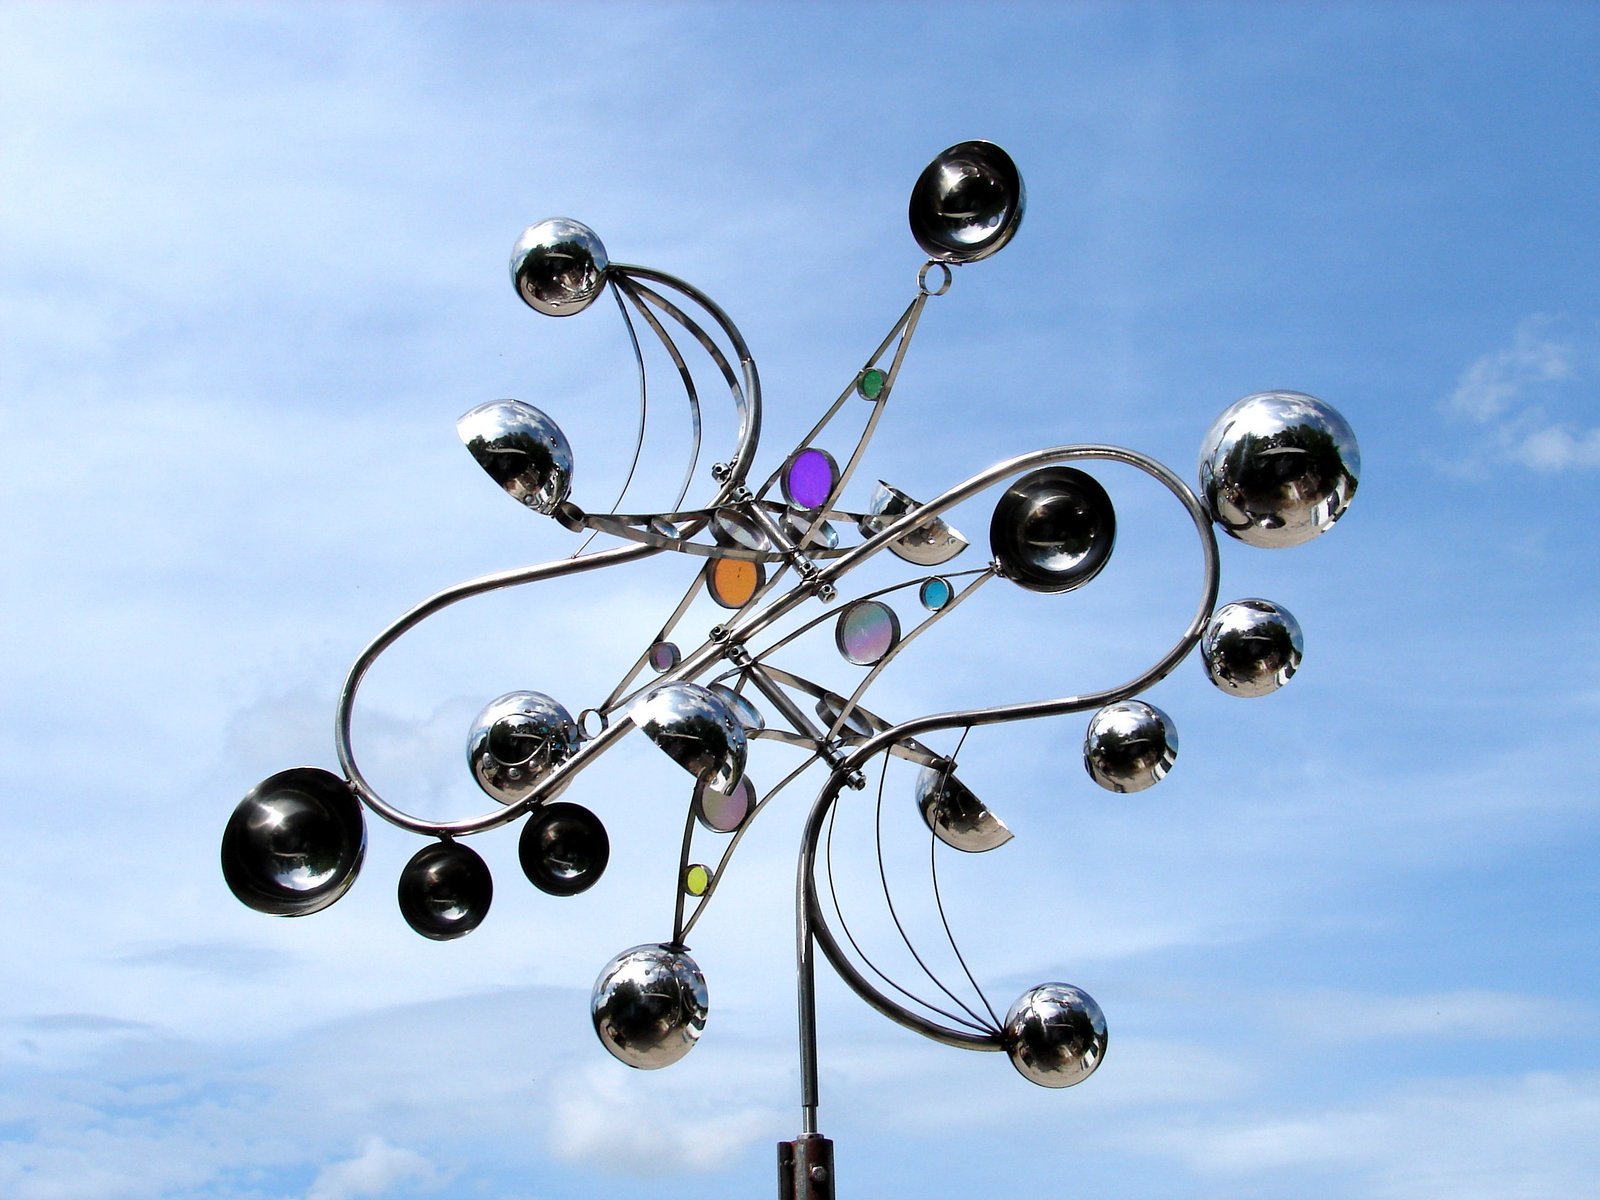
\includegraphics[width=3in]{ArtworkOne.png}}
  \value	{\$10,000}
  \tinker	{}
  }
  
  \NEW{Item}{\iArtworkTwo}{
  \s\MYname	{To Incite}
  \s\MYnumber	{7743}
  \s\MYtext	{Masterful oil painting in bold strokes. Heavily inspired by the classical but looks to be fairly new.\\ 
 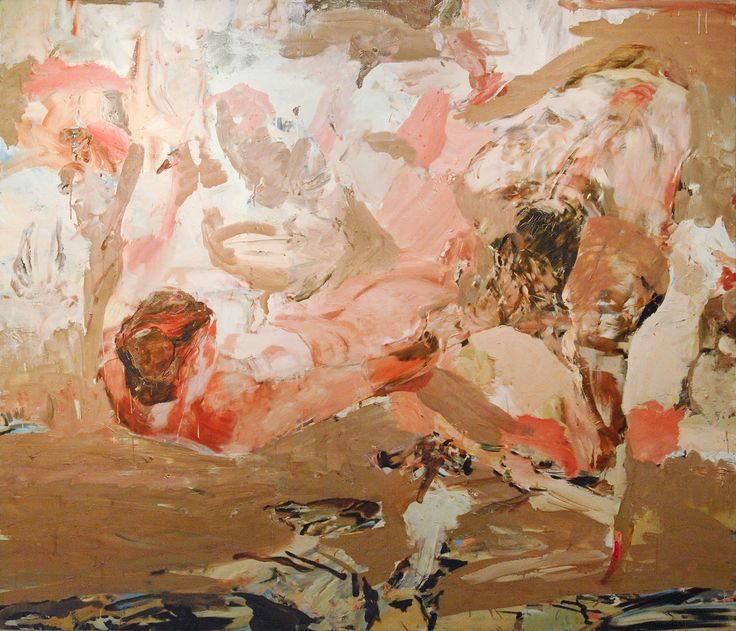
\includegraphics[width=3in]{ArtworkTwo.png}}
      \value	{\$30,000}
  \bulky	{2}
  }
  
  \NEW{Item}{\iArtworkThree}{
  \s\MYname	{Map Key}
  \s\MYnumber	{8065}
  \s\MYtext	{A mesmerizing installation made of 1962 colored keys.\\ 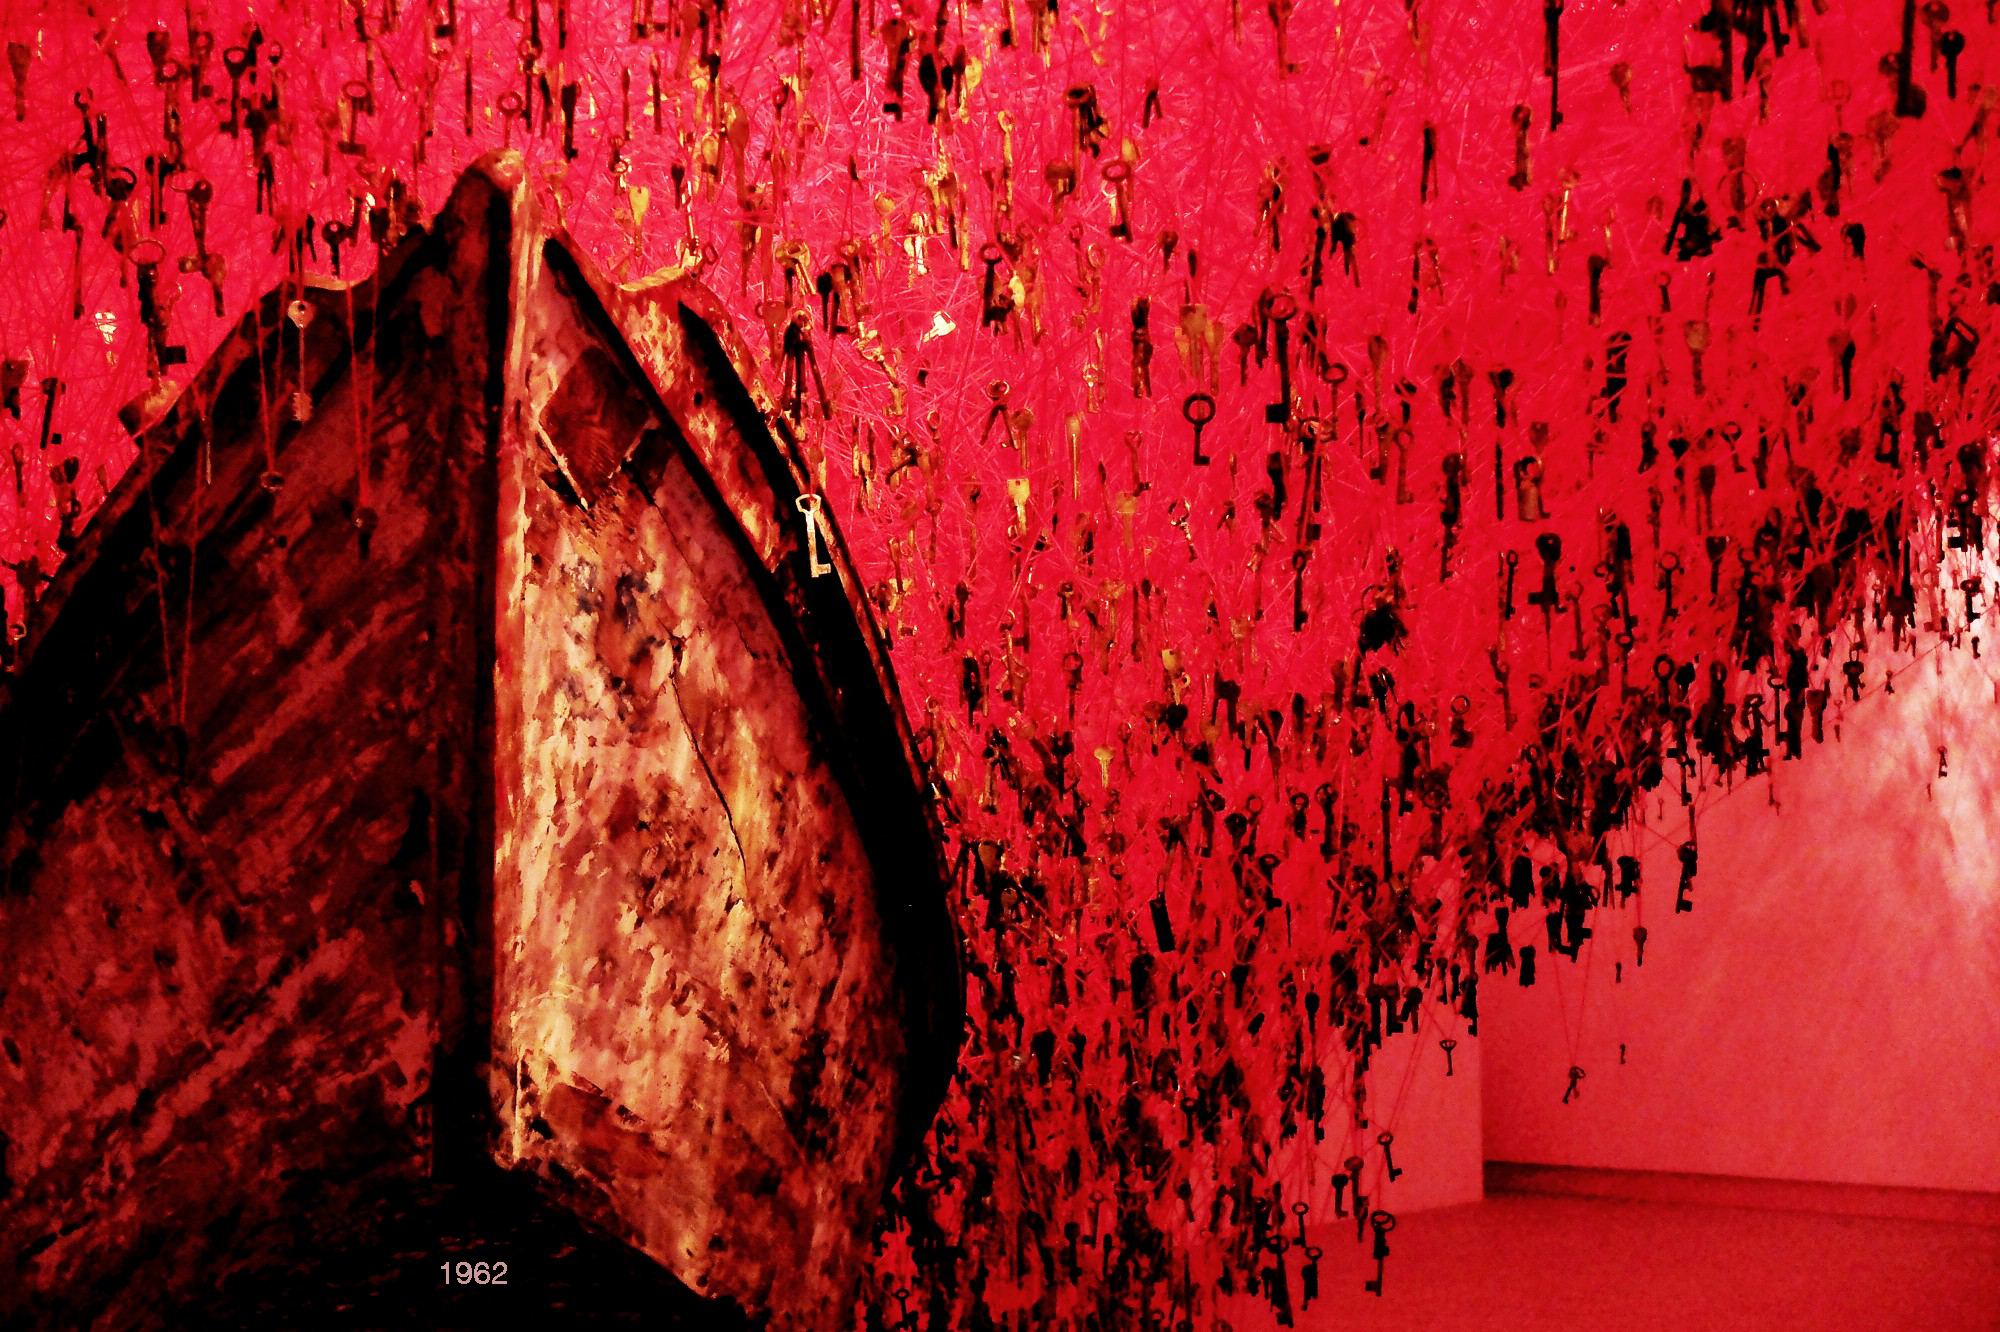
\includegraphics[width=3in]{ArtworkThree.png}}
      \value	{\$20,000}
  }
  
  \NEW{Item}{\iTinkerObjectOne}{
  \s\MYname	{Vintage Record Player}
  \s\MYnumber	{6964}
  \s\MYtext	{Fancy record player with large brass horn and legs, mother of pearl dials. Looks like it hasn't been used in a while.}
  \value	{\$10,000}
  \bulky	{2}
  \tinker	{}
  }
  
  \NEW{Item}{\iTinkerObjectTwo}{
  \s\MYname	{Lava Lamp}
  \s\MYnumber	{7102}
  \s\MYtext	{Red and purple lava lamp.}
  \value	{\$10,000}
  \bulky	{1}
  \tinker	{}
  }
  
\NEW{Item}{\iTinkerObjectThree}{
  \s\MYname	{Massage Chair}
  \s\MYnumber	{7462}
  \s\MYtext	{Comfortable-looking chair upholstered in black leather that reclines and massages.}
  \value	{\$10,000}
  \bulky{3}
  \tinker{}
  }  

  \NEW{Item}{\iTinkerObjectFour}{
  \s\MYname	{Projector}
  \s\MYnumber	{7102}
  \s\MYtext	{A movie screen projector.  Possibly \cGrandma{} used this to display her symbol in the clouds once or twice...}
  \value	{\$10,000}
  \bulky	{1}
  \tinker	{}
  }
  
  \NEW{Item}{\iTinkerObjectFive}{
  \s\MYname	{Speaker system}
  \s\MYnumber	{7102}
  \s\MYtext	{\cGrandma{}'s speaker system.  Possibly used to play her theme song during some of her kapers, er, capers.}
  \value	{\$10,000}
  \bulky	{1}
  \tinker	{}
  }
  
%\NEW{Item}{\iWhatzit}{
%  \s\MYname	{Whatzit}
%  \s\MYnumber	{12345}
%  \s\MYtext	{If you press it, open packet a.  If you twirl it, open
%		packet b.  If you pull it, open packet c.}
%  \bulky	{1}
%  \s\MYsigns	{\signstrip{a}{it goes ``beep.''}
%		\signstrip{b}{it goes ``whoop.''}
%		\signstrip{c}{it goes ``bang.''}
%		}
 % \s\MYabils	{\ability{Stop Crying}{By futzing with the Whatzit, you
%		can make babies stop crying.}{I make the baby stop
%		crying.}
%		}
 % }


%%%%%%%%%%%%%%%%%%%%%%%%%%%%%%%%%%%%%%%%%%%%%%%%%%%%%%%%%%%%%%%%%%



%%%%%%%%%%%%%%%%%%%%%%%%%%%%%%%%%%%%%%%%%%%%%%%%%%%%%%%%%%%%%%%%%%
